\section{Illustration of the system}
The idea with making a rich picture is to get an understanding about the current interaction with technology. This is an overview of how the users who are the guardian and pedagogue and the child would interact with the mobile device. Under the assumption that the multi-bachelor project has been implemented in the everyday life to show how it could be improved with an administrator program on the computer.

In the current system the administrator who has the task of administrating the setting, program and data on the mobile device, now also has to be done on the mobile device. At the same time the child also have tasks on the mobile device which then create a problem between child and administrator when they need the mobile device at the same time. The mobile device is used by the child as a communication tool so the administrators are able to understand what the child wants or needs. Though this understanding the child and administrator can easier communicate in their everyday life.

The current problem with the mobile device is that both the administrator and child need it and some children would consider the mobile device theirs and therefore wound not hand it over to the administrator. To resolve this problem and computer program could be made from where the administrator could change the setting and data which then via Wireless Internet and a server then could administrate the mobile device. This picture is shown in \vref{fig:Rig billede}. 

\begin{figure}[h]
	\centering
		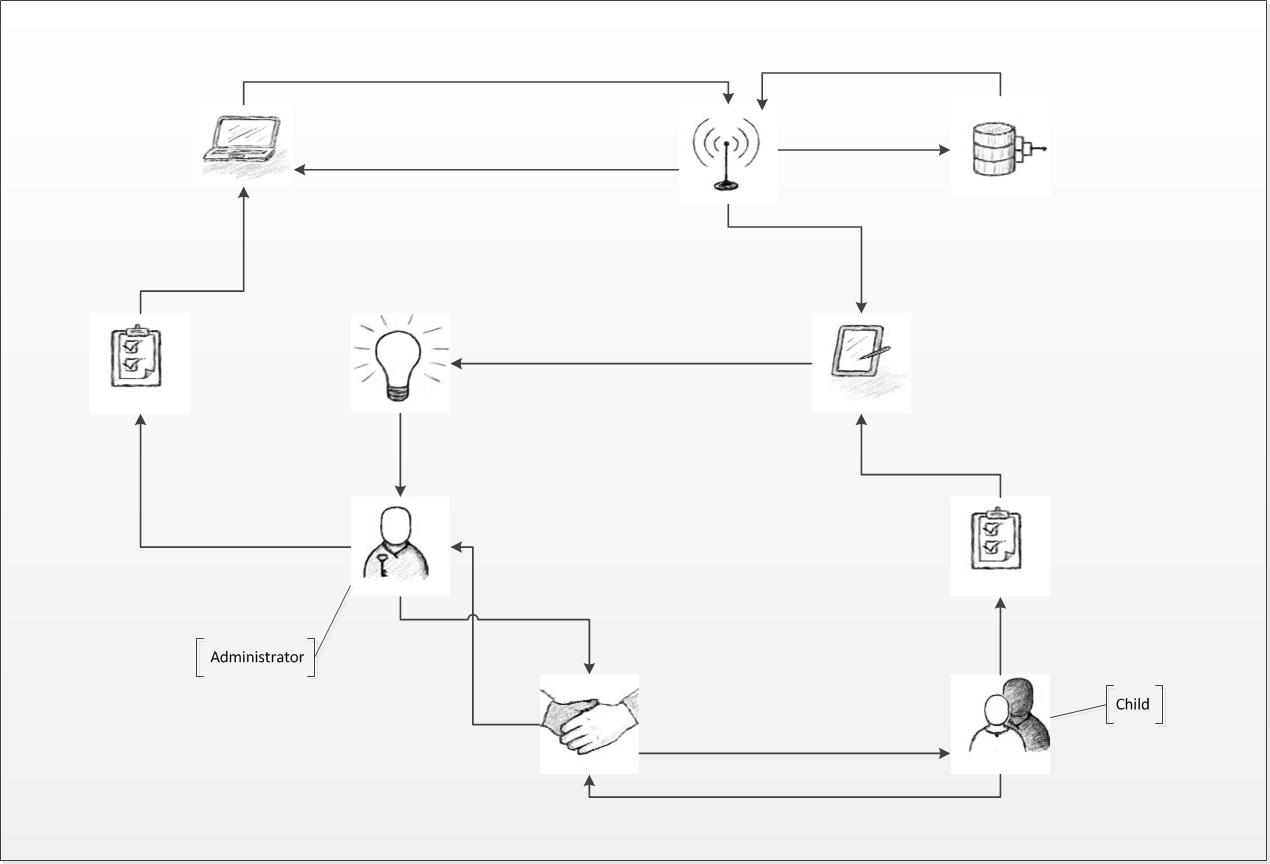
\includegraphics[width=1.00\textwidth]{img/Rig_billede.jpg}
	\caption{How the solutions should be}
	\label{fig:Rig billede}
\end{figure}

In our project we also want to make a digitized version of the contact book such that the guardian and parents easily and quickly can send small messages to each other. Furthermore the guardians would be able to send a summary of what the child have been doing today and include pictures of the child doing an activity. This is the base for our system definition.    